\documentclass[
    a4paper,
    14pt,
    captions=tableheading,
    russian
]{scrreprt}

% Остальные стандартные настройки убраны в preamble.inc.tex.
%Package extsizes not only changes the fontsize, but also amends various skips as well as the margins.
%Changing the page geometry after loading the package will give fixed margins.
%\usepackage{extsizes}

%fonts and localization
\usepackage[utf8]{inputenc}
\usepackage{fontspec}
\RequirePackage{polyglossia}
\providehyphenmins{russian}{{3}{3}}
\setdefaultlanguage[babelshorthands=true,spelling=modern]{russian}
\setotherlanguage{english}
\setmainfont{Liberation Serif}
\setsansfont{Liberation Sans}
\setmonofont{Liberation Mono}
\newfontfamily\cyrillicfont{Liberation Serif}
\newfontfamily\cyrillicfontsf{Liberation Sans}
\newfontfamily\cyrillicfonttt[Scale=0.8]{Liberation Mono}
\defaultfontfeatures{Ligatures=TeX}
\defaultfontfeatures{Mapping=tex-text}

%math
\usepackage{amssymb}
\usepackage{amsmath}
%for \degree
\usepackage{gensymb}

% table of contents
\usepackage[tocflat]{tocstyle}

% bibliography
\usepackage[parentracker=true,
            backend=biber,
            language=auto,
            autolang=other,
            hyperref=auto,
            citestyle=gost-numeric,
            bibstyle=gost-numeric]
            {biblatex}
\DefineBibliographyStrings{russian}{
    bibliography = {Список использованных источников},
    references = {Список использованных источников}
}
\addbibresource{my.bib}
%disable uri encoding
\usepackage{hyperref}
\DeclareFieldFormat{url}{%
  \mkbibacro{URL}\addcolon\space
  \href{#1}{\nolinkurl{\thefield{urlraw}}}}

%setting page geometry
\usepackage[
a4paper, includefoot,
left=3cm, right=2cm, top=2cm, bottom=1.5cm,
headsep=1cm, footskip=1cm
]{geometry}

%not sure abt this
\usepackage{csquotes}
%quotations
\usepackage[
    left = «,%
    right = »,%
    leftsub = „,%
    rightsub = “%
]{dirtytalk}

%use \input for files. used with latexmk
\newcommand\inputfile[1]{%
    \InputIfFileExists{#1}{}{\typeout{No file #1.}}%
}

% line spacing
\usepackage[nodisplayskipstretch]{setspace}
\setstretch{1.5}

%pictures
\usepackage{graphicx}
\graphicspath{{img/}}
\DeclareGraphicsExtensions{.png,.jpg,.gif}

% \includepdf
\usepackage{pdfpages}

%disable hyphenation
%\disablehyphenation

%justifying
\usepackage{ragged2e}

%paragraph indent
\setlength{\parindent}{1.25cm}
\usepackage{indentfirst}

%titles
\newcommand*{\justifyheading}{\centering}
\usepackage[explicit]{titlesec}

\titleformat{\chapter}[display]
  {\normalfont\justifyheading\bfseries}
  {\thechapter}{1em}{\MakeUppercase{#1}}
  \titlespacing*{\chapter}{\parindent}{-18pt plus 4pt minus 2pt}{30pt plus 4pt minus 2pt}

\titleformat{\section}
  {\normalfont\bfseries}
  {\thesection}{1em}{#1}
  \titlespacing*{\section}{\parindent}{12pt plus 4pt minus 2pt}{12pt plus 4pt minus 2pt}

\titleformat{\subsection}
  {\normalfont\bfseries}
  {\thesubsection}{1em}{#1}
  \titlespacing*{\subsection}{\parindent}{12pt plus 4pt minus 2pt}{12pt plus 4pt minus 2pt}

\titleformat{\subsubsection}
  {\normalfont}
  {\thesubsubsection}{1em}{#1}
  \titlespacing*{\subsubsection}{\parindent}{12pt plus 4pt minus 2pt}{12pt plus 4pt minus 2pt}

%setting numeration
\renewcommand\thesection{\arabic{section}}
\renewcommand\thesubsection{\thesection.\arabic{subsection}}
\renewcommand\thesubsubsection{\thesubsection.\arabic{subsubsection}}
\setcounter{secnumdepth}{3}

%setting lists margin
\usepackage{enumitem}
%\setlist{nosep,leftmargin=\parindent}
\setlist{left=0pt .. \parindent,nosep}
%\setlist{labelindent=\parindent,leftmargin=*,nosep}

\usepackage{float}
%itemize separator
\renewcommand{\labelitemi}{—}
\renewcommand{\labelitemii}{—}
\renewcommand{\labelitemiii}{—}

\usepackage{chngcntr}
\counterwithin{equation}{section}
%tables and figures https://habr.com/ru/post/144648/
\usepackage[
    singlelinecheck=false, %for caption to be aligned left
    tableposition=top,
    figurewithin=section,tablewithin=section] %see chngcntr below
{caption}
\usepackage{subcaption}
\DeclareCaptionLabelFormat{gostfigure}{Рисунок #2}
\DeclareCaptionLabelFormat{gosttable}{Таблица #2}
\DeclareCaptionLabelSeparator{gost}{~—~}
\DeclareCaptionLabelFormat{continued}{Продолжение таблицы~#2}
\captionsetup{labelsep=gost}
\captionsetup[figure]{justification=centering,labelformat=gostfigure}
\captionsetup[table]{justification=raggedright,labelformat=gosttable}

\renewcommand{\thefigure}{\thesection.\arabic{figure}}
\renewcommand{\thesubfigure}{\asbuk{subfigure}}
\renewcommand{\thetable}{\thesection.\arabic{table}}
\renewcommand{\theequation}{\thesection.\arabic{equation}}

%\usepackage[notindex,nottoc]{tocbibind}

\usepackage{array, multirow, makecell}
\usepackage{pgfplotstable}
\usepackage{booktabs}

\usepackage{xtab}
\usepackage{etoolbox}
\makeatletter
\patchcmd{\estimate@lineht}{1\p@}{-2.5\p@}{}{}
\makeatother
% в \tablefirsthead{\shrinkheight{-\normalbaselineskip}}

\usepackage{paracol}
\setcellgapes{4pt}
\makegapedcells

\emergencystretch=15pt

\usepackage{verbatim}
\usepackage{desclist}


\begin{document}

%\begin{center}
    \MakeUppercase{Министерство рогов и копыт}\\
    Федеральное государственное бюджетное образовательное учреждение
    высшего образования \say{Университет Пушкина}\\
    Кафедра Колотушкина\\
    Учебная дисциплина \say{Конструирование конструкторов}\\
    \hfill\break
    \hfill\break
    \hfill\break
    \hfill\break
    \hfill\break
    Лабораторные работы\\
    Прикольные и полезные (нет)\\
    \hfill\break
    \hfill\break
\end{center}

%\hfill\begin{minipage}{0.5\linewidth}
\begin{flushright}
    Выполнил: студент\\
    Группа: группа \\
    \underline{\hspace{3cm}} \\
    Проверил: преподаватель\\
    \underline{\hspace{3cm}} \\
    \say{\underline{\hspace{1cm}}} \underline{\hspace{2cm}} \the\year\\
\end{flushright}
%\end{minipage}
\hfill\break
\hfill\break
\begin{center}
    Городок\\
    \the\year
\end{center}
\thispagestyle{empty} % выключаем отображение номера для этой страницы

% КОНЕЦ ТИТУЛЬНОГО ЛИСТА

\newpage


\setcounter{page}{7} % номер страницы оглавления. Может быть полезным при использовании не родного титульного
\tableofcontents
\thispagestyle{empty} % выключаем отображение номера для этой страницы

%paragraph indent
\setlength{\parindent}{1.25cm}

\clearpage
\addcontentsline{toc}{chapter}{Определения и сокращения}
\chapter*{Определения и сокращения}

В настоящей выпускной квалификационной работе используются следующие термины, сокращения
и обозначения с соответствующими определениями:

%\renewcommand{\descriptionlabel}[1]{\hspace{\labelsep}{#1}}

\noindent
	\begin{desclist}{}{ \rm\hfill —}[ПО]
		\item[БД] база данных
        \item[Дистрибутив] форма распространения программного обеспечения
        \item[Локальная вычислительная сеть (ЛВС)] частная сеть, размещенная, как
            правило, в одном здании или на территории одной организации
		\item[ОС] операционная система
		\item[ПАК] программно-аппаратный комплекс
		\item[ПК] персональный компьютер
		\item[ПО] программное обеспечение
        \item[САПР] система автоматизированного проектирования
		\item[ТК] тонкий клиент, терминал, устройство терминального доступа
		\item[Ethernet] семейство технологий пакетной передачи данных между
	устройствами для компьютерных и промышленных сетей. Ethernet в основном
	описывается стандартами IEEE группы 802.3
        \item[Linux] семейство Unix-подобных операционных систем на базе ядра Linux,
            включающих тот или иной набор утилит и программ, и, возможно,
            другие компоненты. 
        \item[Local Area Network (LAN)] локальная вычислительная сеть
        \item[Remote Desktop Protocol (RDP)] протокол удаленного доступа, используемый в
            ОС семейства Windows.
	\end{desclist}

\clearpage
\addcontentsline{toc}{chapter}{Введение}
\chapter*{Введение}

С развитием вычислительной техники системные требования программного обеспечения
становятся все более высокими. За последнее время производительность компьютеров
значительно выросла, поэтому старые устройства уже не справляются с современными
программами, особенно с требовательными САПР, используемыми в учебном процессе
на кафедре КПРС.

Актуальность работы состоит в том, что новые версии таких САПР, как SolidWorks 2019 и
Altium Designer 19, неудовлетворительно работают на компьютерах кафедры.
При модернизации компьютерных классов есть
возможность использовать подход к организации сети, основанный на тонких клиентах —
терминальных станциях, которые подключаются к производительному серверу, на котором
производятся вычисления.

Целью выпускной квалификационной работы является разработка общевычислительного
многопользовательского программно-аппаратного комплекса (ПАК) на основе тонких клиентов.

Объектом исследования является вычислительный комплекс кафедры.

Предмет исследования — модернизация вычислительного комплекса.

Для достижения заданной цели были поставлены следующие задачи:

\begin{enumerate}
    \item Рассмотреть технологии организации вычислительных сетей
    \item Разработать проект программно-аппаратного комплекса
    \item Установить и настроить комплекс
    \item Проанализировать результаты работы
\end{enumerate}

Практическая значимость работы состоит в том, что вычислительный комплекс кафедры может
быть модернизирован в соответствии с выдвигаемыми в работе предложениям, по прописанным
пошаговым инструкциям.

В первой главе рассматриваются основные технологии организации вычислительных сетей.

Во второй главе разрабатывается проект ПАК, выбирается программное и аппаратное
обеспечение.

В третьей главе описывается процесс установки и настройки комплекса, разрабатывается
корпус для изделия.

В четвертой главе анализируются результаты работы, исследуется производительность и
экономическая эффективность, проводится анализ на устойчивость к внешним воздействиям.

В заключении формулируются выводы и предложения по использованию результатов работы.

\clearpage
\chapter{Обзор технологий организации вычислительных сетей}

\section{Определение локальных сетей}

Локальными сетями называют частные сети, размещающиеся, как правило, в одном здании или
на территории какой-либо организации. Их часто используют для объединения компьютеров и
рабочих станций в офисах компании или предприятия бытовой электроники для предоставления
совместного доступа к ресурсам (например, принтерам) и обмена информацией
\cite{tanenbaum}. Важными требованими, предъявляемыми к ЛВС, являются:

\begin{itemize}
    \item Низкий уровень ошибок передачи, вызванных внутренними или внешними факторами.
        Допустимая вероятность ошибок передачи данных должна быть порядка
        $10^{-8}$–$10^{-12}$.
    
    \item Возможность  работы  с  большими нагрузками  или высокая интенсивность обмена.
        Если механизм управления в сети не эффективен, то компьютеры могут подолгу ждать
        свою очередь на передачу. И даже если передача будет на высочайшей высоте и
        безошибочна, задержка доступа пользователю данной сети будет неприемлема.
\end{itemize}

Большинство ЛВС имеет выход в глобальную сеть. Но характер информации,  принципы
организации  обмена,  режимы  доступа  к  ресурсам внутри (ЛВС), как правило, отличаются
от принципов, принятых в глобальной сети. Возможность выхода в глобальную сеть — это
лишь один из ресурсов, разделяемых пользователями ЛВС. По ЛВС могут передаваться:
данные, изображения, телефонные разговоры, электронные письма и т.д. Чаще всего ЛВС
используются для совместного использования дискового пространства, принтеров и факсов,
выхода в глобальную сеть, но это лишь часть тех возможностей, которые предоставляют ЛВС. 

Например,  они  позволяют  осуществлять  обмен  информацией между
компьютерами  разных типов. ЛВС дают возможность организовать систему параллельных
вычислений на всех компьютерах сети, что ускоряет решение сложных задач. С их помощью,
можно управлять работой техноло-гической системы или исследовательской установки с
нескольких компью-теров одновременно. Однако ЛВС имеют ряд существенных недостатков:

\begin{itemize}
    \item ЛВС требует дополнительных, иногда значительных материальных затрат на
        покупку сетевого оборудования, ПО, на прокладку кабелей и обучение персонала. 
    \item ЛВС требует приема на работу специалиста (администратора сети),  который
        будет контролировать  работу сети, модернизировать, управлять доступом к
        ресурсам, устранять возможные неисправности, защищать информацию и делать
        резервные копии. Для больших сетей может понадобиться целая бригада
        специалистов. ЛВС ограничивает перемещение компьютеров, подключенных к ней, так
        как при этом требуется перекладка соединительных кабелей.
    \item ЛВС являются прекрасной средой для распространения компьютерных  вирусов,
        поэтому придется уделять  много  времени  вопросу о защите от них. Все
        компьютеры сети могут быть заражены, если заразить всего один.
    \item ЛВС резко повышают опасность несанкционированного доступа к информации с целью
        ее кражи или уничтожения. Информационная защита требует проведения комплекса
        технических и организационных мероприятий.
\end{itemize}

ЛВС классифицируются,  прежде  всего, по протоколам  1-го  и  2-го уровней OSI, то есть,
по технологии используемого сетевого оборудования: Ethernet, Token Ring, FDDI,
AppleTalk. По масштабам и иерархии построения ЛВС различают: 
\begin{itemize}
    \item сети рабочих групп (5-20 станций); 
    \item сети отделов (20-100 станций); 
    \item сети предприятий (корпоративные сети).
\end{itemize}

Последние имеют  развернутую структуру  сетевых  служб  и  по  географии могут выходить
за рамки локальных сетей, образуя кампусные сети, сети с удаленным доступом, а также
сети других масштабов, вплоть до корпоративных частных глобальных сетей. Количество
станций в корпоративных сетях варьируется: от 20 компьютеров до десятков тысяч.

\begin{figure}[h]
    \center
    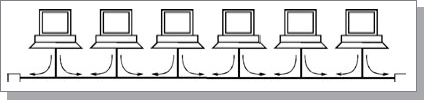
\includegraphics[width=0.7\linewidth]{topo_bus}
    \caption{Топология {шина}}
    \label{pic:topo_bus}
\end{figure}
\begin{figure}[h]
    \center
    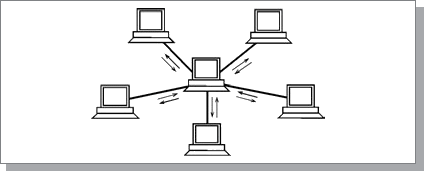
\includegraphics[width=0.7\linewidth]{topo_star}
    \caption{Топология {звезда}}
    \label{pic:topo_star}
\end{figure}
\begin{figure}[h]
    \center
    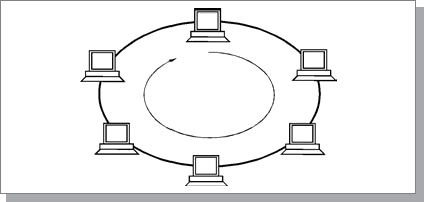
\includegraphics[width=0.7\linewidth]{topo_ring}
    \caption{Топология {кольцо}}
    \label{pic:topo_ring}
\end{figure}

Для организации сетей используются различные топологии. Основных топологии, применяемые
в ЛВС, такие: 

Шина (bus) — все устройства параллельно подключаются к одной линии связи. Информация
от каждого устройства одновременно передается всем остальным
(см. рисунок \ref{pic:topo_bus}).

Звезда (star) — к одному центральному устройству присоединяются остальные периферийные
устройства, причем каждый из них использует отдельную линию связи. Информация
от периферийного устройства направляется только центральному, а от него —
одному или нескольким периферийным
(см. рисунок \ref{pic:topo_star}).

Кольцо (ring) — устройства последовательно объединены в кольцо. Передача информации
в кольце всегда производится только в одном направлении. Каждое из устройств
передает информацию только одному следующему в цепочке за ним, а
получает информацию только от предыдущего в цепочке.
(см. рисунок \ref{pic:topo_ring}).

В зависимости от характера распределения функций различают: 

\begin{itemize}
    \item одноранговые  сети — небольшие  локальные  сети,  в которых компьютеры являются
        равноправными; обычно включают в себя до 15 станций;

    \item сети с выделенными серверами (двухранговые сети) — средние и крупные сети, в
        которых часть выполняемых функций обслуживания станций возложена на серверы. Такие
        сети характеризуются типами  используемых в них сетевых служб: файловая служба,
        служба печати, служба терминалов, управление базами данных, Web-служба, почтовая
        служба, службы интерактивного общения, прокси-сервер, сетевая безопасность.
\end{itemize}


\subsection{Архитектуры вычислительных сетей}

Вычислительные системы имеют два основных вида построения архитектуры: централизованный
и распределенный (также называемый клиент-сервер).

Основное различие между ними состоит в том, что в централизованной архитектуре большая
часть вычислений происходит на сервере. В распределенной системе все машины имеют
одинаковое назначение и все занимаются вычислениями.

Система клиент-сервер состоит из двух типов взаимодействующих устройств (см.
рисунок~\ref{pic:client-server}).
В большинстве случаев взаимодействие происходит по следующей модели:

\begin{enumerate}
    \item Клиент отправляет запрос на получение данных серверу;
    \item Сервер, получив запрос, начинает обработку данных, различные расчеты и т.п.
        (в зависимости от назначения сервера);
    \item Сервер отправляет обработанные или новые данные клиенту.
\end{enumerate}

\begin{figure}[h]
    \center
    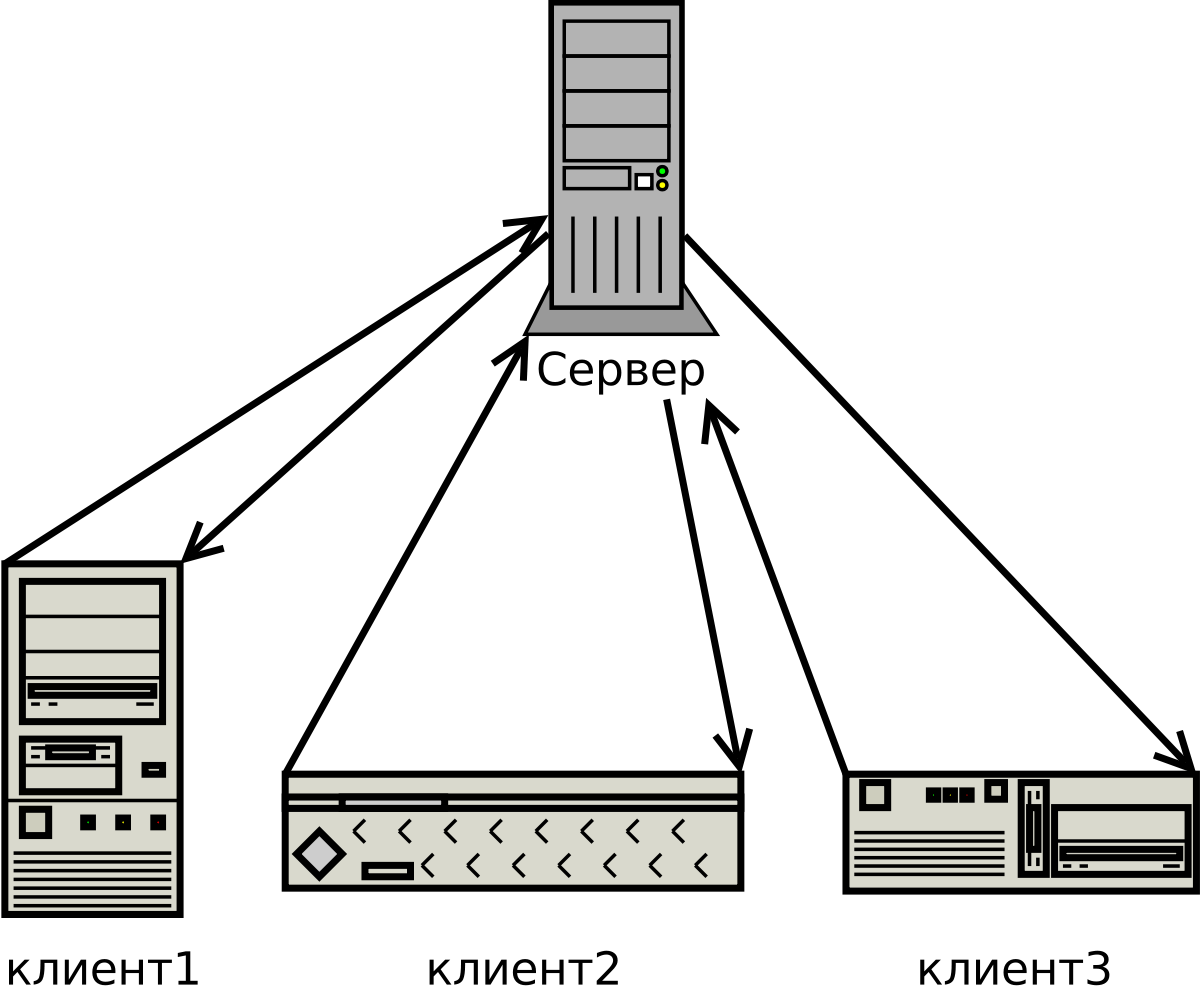
\includegraphics[height=9cm]{client-server}
    \caption{Клиент-серверная архитектура}
    \label{pic:client-server}
\end{figure}

\begin{figure}[h]
    \center
    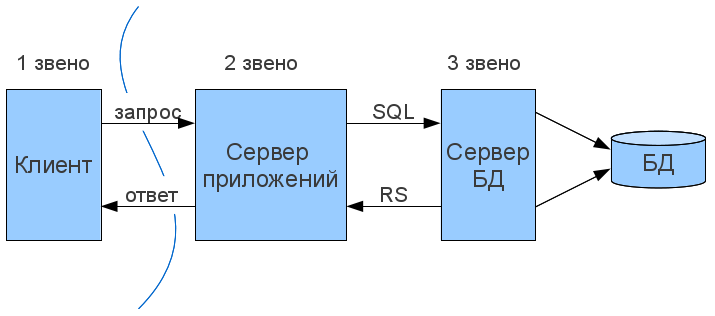
\includegraphics[height=5cm]{client-server-db}
    \caption{Клиент-серверная архитектура с разделением серверов}
    \label{pic:client-server-db}
\end{figure}

В настоящее время в сетях с централизованной архитектурой может быть применен принцип
разделения обязанностей серверов. Например, разделение серверов приложений, баз данных и
вычислений (см. рисунок~\ref{pic:client-server-db}).


\subsection{Терминальные системы}
Первые компьютеры 50-х годов предназначались для очень небольшого числа избранных
пользователей. Такие компьютеры не были предназначены для интерактивной работы
пользователя, а применялись в режиме пакетной обработки.  Задания нескольких
пользователей группировались в пакет, который принимался на выполнение. Распечатанные
результаты пользователи получали обычно только на следующий день.

По мере удешевления процессоров в начале 60-х годов появились новые способы организации
вычислительного процесса, которые позволили учесть интересы пользователей.  Начали
развиваться интерактивные многотерминальные системы разделения времени.  В таких
системах каждый пользователь получал собственный терминал, с помощью которого он мог
вести диалог с компьютером.
Действительно, рядовой пользователь работу за терминалом мэйнфрейма воспринимал примерно
так же, как сейчас он воспринимает работу за подключенным к сети персональным
компьютером. Пользователь мог получить доступ к общим файлам и периферийным устройствам,
при этом у него поддерживалась полная иллюзия единоличного владения компьютером, так как
он мог запустить нужную ему программу в любой момент и почти сразу же получить
результат. \cite{olifer}

Дальнейшее развитие информационных технологий и удешвление персональных компьютеров
привело к падению релевантности терминальных систем. Однако, в настоящее время тип
организации сетей, в основе которого лежат терминалы, называемые "тонкими клиентами" (в
противовес "толстым клиентам" — обычным ПК), вновь набирает популярность. Из-за
увеличения числа ПК в сетях их обслуживание становится все более сложным. Поэтому тонкие
клиенты стали снова широко использоваться.

\section{Система тонких клиентов}
Тонкий клиент, как и классический терминал 50–60-х годов, дает пользователю возможность
взаимодействия с удаленным компьютером. Разница в том, что если мощностей терминалов,
мэйнфреймов и пропускной способности сети хватало только для отправки текстовых команд и
получения текстовых результатов, то современные тонкие клиенты позволяют пользователям
взаимодействовать и с графическими интерефейсами, работать с графикой и даже
воспроизводить видео. Для пользователя тонкого клиента взаимодействие с удаленным
рабочим столом должно выглядеть неотличимо от обычного ПК. Современные ТК позволяют это
сделать.

Система, основанная на тонких клиентах, состоит из терминального сервера и одного и
более ТК. На терминальном сервере установлена ОС, позволяющая подключение ТК. Все
клиенты настроены на подключение к этому серверу и занимаются только вводом-выводом
информации для взаимодействия с пользователем, и выполнением протоколов удаленного
доступа. Все вычисления, работа ОС и процессов, взаимодействие с устройствами хранения
информации выполняются на сервере. 

Таким образом, все ресурсоемкие процессы в системе ТК перенесены на сервер. Это
означает, что для клиентских машин нужно минимальное аппаратное обеспечение, достаточное
для вывода изображения на экран, работы с сетью и устройствами ввода-вывода. В качестве
таких клиентов могут выступать как специализированные устройства, так и устаревшие ПК,
мощности которых уже не хватает для привычных пользователям задач.
(см. рисунок~\ref{pic:PCtoTC}).

\begin{figure}[htpb]
    \center
    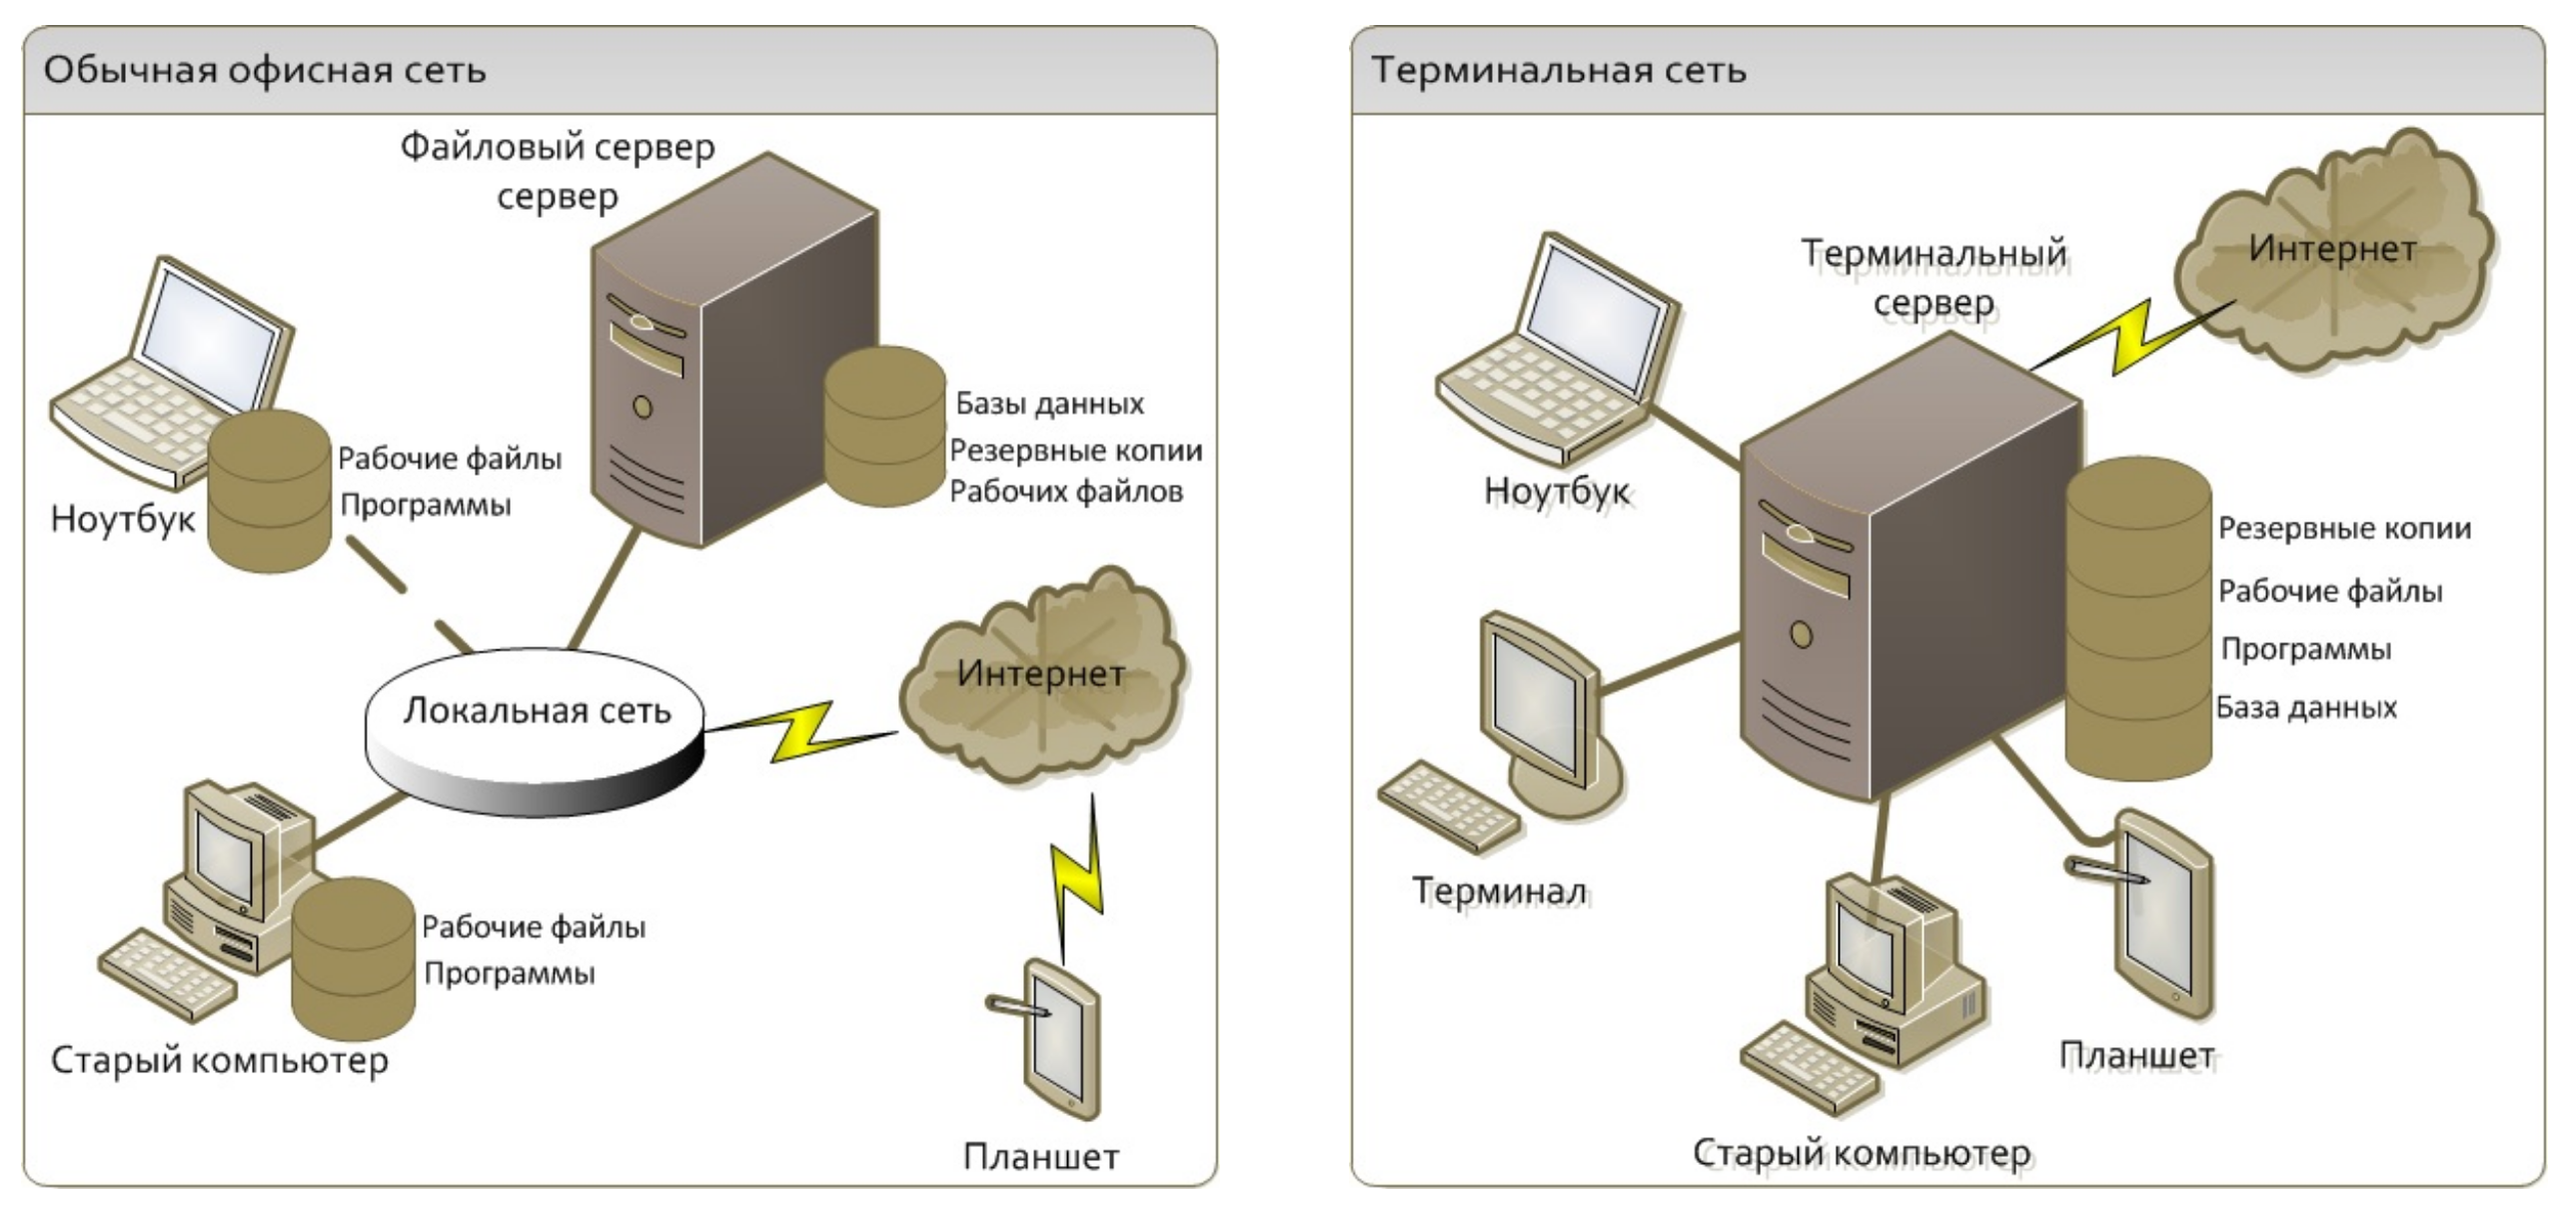
\includegraphics[width=\linewidth]{PCtoTC}
    \caption{Сравнение типовой и терминальной сетей. Источник: \cite{PCtoTCsrc}}
    \label{pic:PCtoTC}
\end{figure}

Преимущества систем, построенных на базе тонких клиентов:
\begin{itemize}
    \item   Экономия средств. Необходимость в постоянной модернизации всего парка
        компьютеров с выходом более новых и ресурсоёмких ОС и приложений исчезает.
        Модернизировать, при необходимости, нужно будет только терминальный сервер и
        серверы БД; терминалы не нуждаются в модернизации в течение длительного времени
        (7-10 лет). Лицензия терминального доступа стоит дешевле настольной ОС, не нужны
        локальные антивирусы, сложное ПО управления парком ПК, что значительно сокращает
        затраты. Снижается количество рутинных операций, а также перемещений IT
        персонала для обслуживания подразделений. При использовании терминала нет
        необходимости дополнительно приобретать источник бесперебойного питания для
        защиты от внезапного отключения питания, вся информация остается доступной на
        серверах. Даже при аппаратной замене ТК пользователь может продолжить работу.
    \item   Надежность. Использование серверной операционной системы и аппаратуры
        сервера повышает надежность работы и хранения данных. Выход из строя терминала,
        его утрата не повлекут за собой потерю или порчу данных на сервере.
    \item   Безопасность. Отсутствие на клиентских машинах жестких дисков, дисководов и
        приводов оптических дисков позволяет избежать несанкционированного копирования и
        выноса данных. Отсутствие непосредственной передачи данных по сети позволяет
        избежать их перехвата. Все программное обеспечение ставится только системным
        администратором. При краже или изъятии обычного компьютера есть риск потерять
        важные конфиденциальные данные, хранящиеся на нем. Терминал гораздо менее
        привлекателен для воров, т.к. не применим в домашних условиях, а при
        использовании тонких клиентов данные на конечном устройстве не хранятся.
    \item   Централизация. Все данные хранятся только на серверах, что упрощает
        процедуру резервного копирования, контроля версий ПО, контроля доступа
        пользователей. Всё ПО находится на серверах - это упрощает администрирование.
        Конечный пользователь не может повлиять на стабильность такой системы.
    \item   Эффективность. Загрузка процессора на ПК в большинстве случаев не превышает
        4-5\%. Терминальная система позволяет максимально полезно использовать
        вычислительные ресурсы сервера, распределяя их между работающими в данный момент
        пользователями.
    \item   Снижение энергопотребления. Тонкие клиенты используют
        энергоэффективные процессоры и не имеют подвижных компонентов, потребляют всего
        около 10\% мощности обычного ПК.
    \item   Тихая работа. Из-за низкого энергопотребления тепловыделение процессоров ТК
        невелико. Это позволяет использовать активные систмы охлаждения с малыми
        скоростями вращения вентиляторов, или использовать полностью пассивные системы
        охлаждения, что обеспечивает бесшумную работу клиентов.
    \item   Быстрое развертывание и обновление приложений. При использовании ТК вы
        просто устанавливаете новое ПО на серверах, и оно становится доступным сотням
        пользователей сразу после публикации.
    \item   Устранение поддержки конечных узлов. ПК – источник аппаратных проблем и
        проблем локальных конфигураций. При использовании ТК отпадает необходимость
        подходить к пользовательским устройствам для настройки системы, установки и
        ремонта программ, помощи в настройке приложений, замены сломанных деталей. ТК
        используют операционную систему терминального сервера, а приложения
        устанавливаются на серверах. Служба техподдержки может помогать пользователям
        посредством удаленного управления их терминальными сеансами. При выходе ТК из
        строя его легко заменить, что может выполнить специально назначенный сотрудник,
        даже не имеющий IT образования.
    \item   Защита от вирусов. Тонкие клиенты не подвержены заражению вирусами, на них
        антивирусное ПО не устанавливается. Достаточно установить антивирусное ПО на
        серверы компании. Локальный ПК не защищен от заражения при сбое параметров
        обновления или настройки антивируса и дальнейшего распространения вируса в ИС.
\end{itemize}

Из существенных недостатков системы на базе ТК можно выделить только необходимость
первоначальной настройки системы. Для внедрения данной системы нужно подготовить
достаточно производительный терминальный сервер, а также настроить его в соответствии с
планируемой архитектурой сети.  Также для корректной работы всей сети администратор
должен знать о ее организации.  Требуется более высокая квалификация администратора,
т.к. в его обязанности также будет входить поддержка протоколов удаленного доступа,
использованных в системе.  Однако, это компенсируется более низкой требуемой
квалификацией техников.

\clearpage
\section{Разработка программно-аппаратного комплекса}

\subsection{Серверная аппаратная часть}
Для выбора серверной аппаратной части нужно опираться, в первую очередь, на системные
требования используемого на кафедре ПО. Для оценки в таблице \ref{tab:solid_req}
приводятся системные требования основного используемого на кафедре КПРС САПР SolidWorks
с сайта разработчика Dassault Systems \cite{ref:solid_req2} \cite{ref:solid_req1}.

\begin{table}[htpb]
    \centering
    \caption{Системные требования Solidworks}
    \label{tab:solid_req}
    \begin{tabularx}{\linewidth}{Xr}
        \toprule
        Процессор & 3.3 ГГц или выше \\
        RAM & 16 ГБ или более \\
            & 32 ГБ рекомендуется для Simulation \\
            & и работы с большими сборками \\
        Устройство хранения & рекомендуется SSD \\
        Место на диске & 20 ГБ и более \\
        \bottomrule
    \end{tabularx}
\end{table}

\subsection{Клиентская аппаратная часть}
Для работы в качестве тонкого клиента подходит практически любой x86-совместимый
компьютер, на котором есть возможность запустить клиент нужного протокола.
Соответственно, существующие на кафедре компьютеры могут быть использованы в качестве
ТК. Однако, для получения многих преимуществ ТК есть смысл использовать более
компактные и энергоэффективные системы.

В качестве основной платформы для разработки ТК будет использован одноплатный компьютер
Raspberry Pi 3B. Его характеристики приведены в таблице \ref{tab:rpi_specs}.
По результатам предварительных исследований, его производительности
достаточно для использования в этом проекте.

\begin{table}[htpb]
    \centering
    \caption{Технические характеристики Raspberry Pi 3B}
    \label{tab:rpi_specs}
    \begin{tabularx}{\linewidth}{Xr}
        \toprule
        Процессор & однокристальный чип Broadcom BCM2837 \\
        микроархитектура & ARM Cortex-A53 \\
        разрядность & 64-бит \\
        количество ядер & 4 \\
        тактовая частота & 1,2 ГГц \\
        оперативная память & 1ГБ LPDDR2 SDRAM \\
        \midrule
        цифровой видеовыход & HDMI \\
        композитный выход & 3,5 мм (4 pin) \\
        USB порты & USB 2.0×4 \\
        сеть & WiFi 802.11n, 10/100 Мб RJ45 Ethernet \\
        Bluetooth & Bluetooth 4.1, Bluetooth Low Energy \\
        разъем дисплея & Display Serial Interface (DSI) \\
        разъем видеокамеры & MIPI Camera Serial Interface (CSI-2) \\
        карта памяти & MicroSD \\
        порты ввода-вывода & 40 \\
        габариты & 85x56x17 мм \\
        \bottomrule
    \end{tabularx}
\end{table}

\subsection{Выбор используемого протокола}

Для разработки необходимо выбрать способ удаленного доступа, который будет
использоваться в системе.

\clearpage
\addcontentsline{toc}{chapter}{Заключение}
\chapter*{Заключение}




\printbibliography[
    heading=bibintoc
]

\end{document}
